\documentclass[12pt,a4paper]{article}

\usepackage[T1]{fontenc}
\usepackage[utf8]{inputenc}
\usepackage[brazil]{babel}
\usepackage{graphicx}
\usepackage{geometry}

\geometry{margin=2.5cm}

\title{Introdução ao \LaTeX{} com TeXstudio}
\author{Adryan Francisco}
\date{\today}

\begin{document}

\maketitle

\section{Introdução}

O \LaTeX{} é um sistema de preparação de documentos muito utilizado na produção
acadêmica por oferecer alta qualidade tipográfica, facilidade de organização e
padronização do conteúdo. Além disso, o uso de ambientes específicos permite
estruturar textos, tabelas, listas e referências de forma clara e consistente.

Segundo \cite{silva2024latex}, a principal vantagem do \LaTeX{} é a separação
entre conteúdo e formatação, o que facilita revisões e reaproveitamento do
material em diferentes contextos.

\section{Desenvolvimento}

Nesta seção, são apresentados alguns elementos básicos exigidos para a criação
de um mini-artigo.

\subsection*{Lista de vantagens}

A seguir, apresenta-se uma lista numerada com exemplos de benefícios do uso do
\LaTeX{}:

\begin{enumerate}
    \item Organização eficiente de documentos longos;
    \item Facilidade para inserir equações, figuras e tabelas;
    \item Geração de arquivos com aparência profissional.
\end{enumerate}

\subsection*{Imagem}

A Figura \ref{fig:fluxo-latex} ilustra um fluxo simplificado de produção de um
documento acadêmico em \LaTeX{}.

\begin{figure}[htbp]
    \centering
    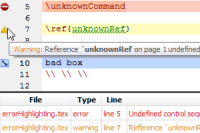
\includegraphics[width=0.8\textwidth]{errorHighlighting_zoom.png}
    \caption{Exemplo visual de destaque de erros no ambiente TeXstudio.}
    \label{fig:fluxo-latex}
\end{figure}

\subsection*{Tabela}

A Tabela \ref{tab:comparacao} apresenta uma comparação simples entre etapas
comuns do processo de escrita acadêmica.

\begin{table}[htbp]
    \centering
    \begin{tabular}{|l|c|c|}
        \hline
        \textbf{Etapa} & \textbf{Objetivo} & \textbf{Status} \\
        \hline
        Planejamento & Definir a estrutura & Concluído \\
        \hline
        Redação & Produzir o conteúdo & Em andamento \\
        \hline
        Revisão & Corrigir e padronizar & Pendente \\
        \hline
    \end{tabular}
    \caption{Exemplo de tabela simples em um documento \LaTeX{}.}
    \label{tab:comparacao}
\end{table}

\section{Conclusão}

O uso do \LaTeX{} com o TeXstudio contribui para a produção de documentos
acadêmicos mais organizados, legíveis e profissionais. Com poucos comandos, é
possível estruturar um artigo com título, seções, listas, figuras, tabelas e
referências bibliográficas, atendendo aos requisitos básicos de trabalhos
acadêmicos.

\begin{thebibliography}{9}

\bibitem{silva2024latex}
Silva, J. R.
\textit{Fundamentos de formatação científica com \LaTeX{}}.
Editora Acadêmica Fictícia, 2024.

\end{thebibliography}

\end{document}
